\chapter{Konzept}
Das folgenden Bild beschreibt den groben Aufbau der Anwendung und die Technologien die auf den verschiedenen Ebenen verwendet wird.
\begin{figure}
	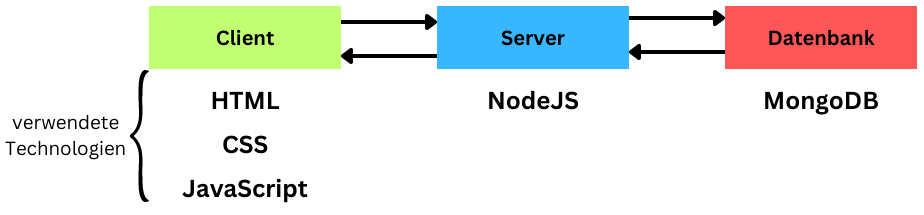
\includegraphics[width=0.8\textwidth]{images/Architektur.png}
	\centering
	\caption{Grobe Architektur des Systems}
\end{figure}

Die Sitemap dient dazu die Navigation durch die  Anwendung und den Zusammenhang der einzelnen Unterseiten darzustellen.
\begin{figure}
	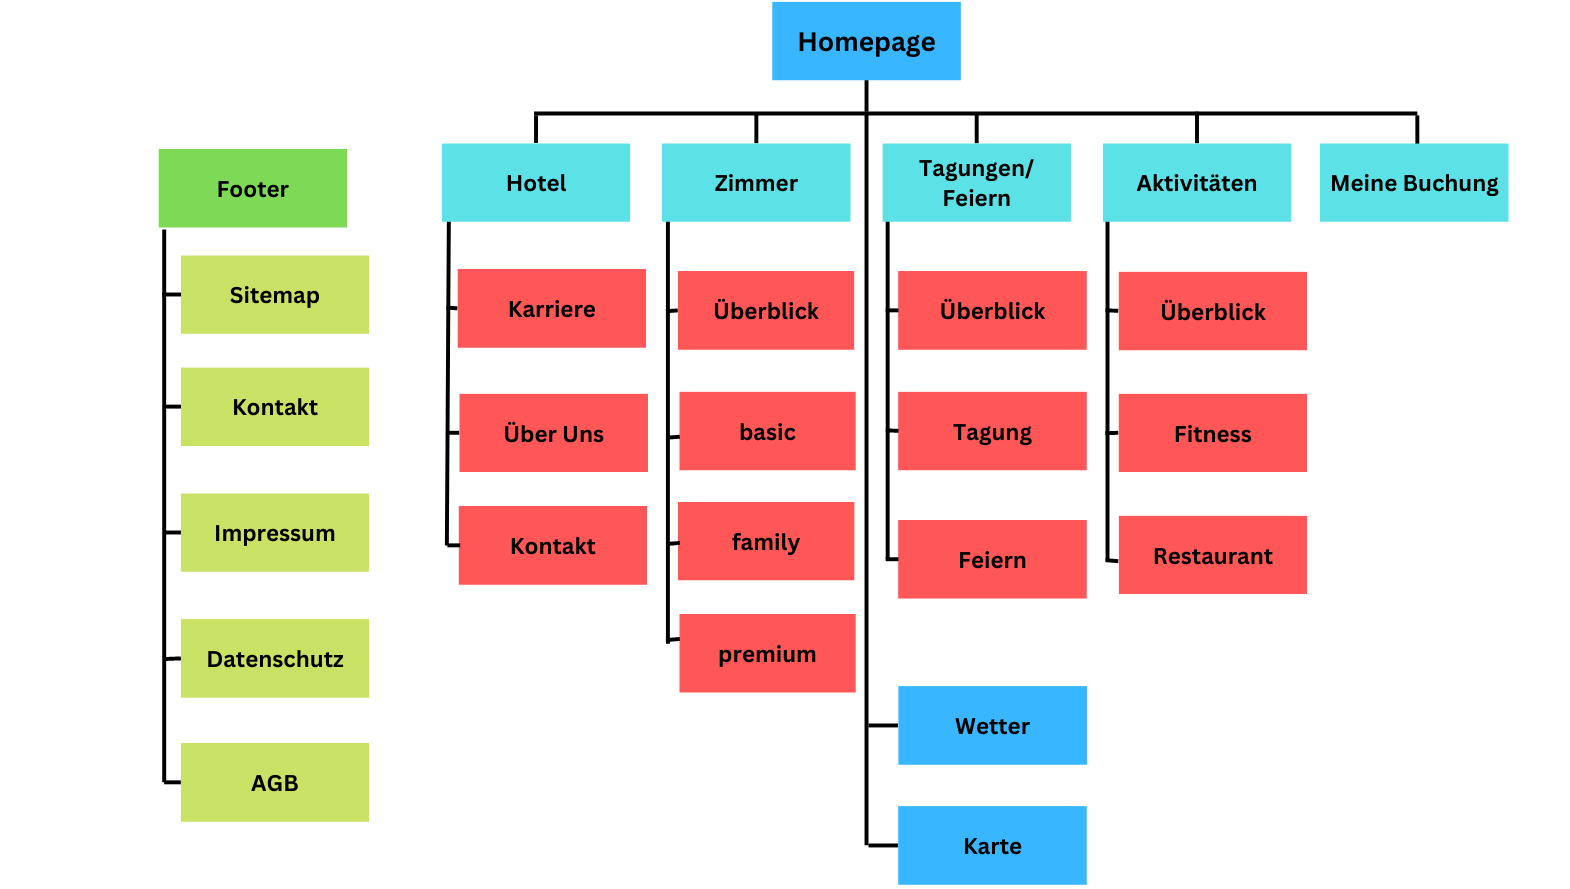
\includegraphics[width=0.8\textwidth]{images/Sitemap.png}
	\centering
	\caption{Sitemap}
\end{figure}
\newpage
Diese Abbildung stellt den Aufbau der Datenbank dar, wobei jedes Rechteck eine Collection abbildet mit Dokumenten die jeweils die Ovale als Attribute besitzt.

\begin{figure}
	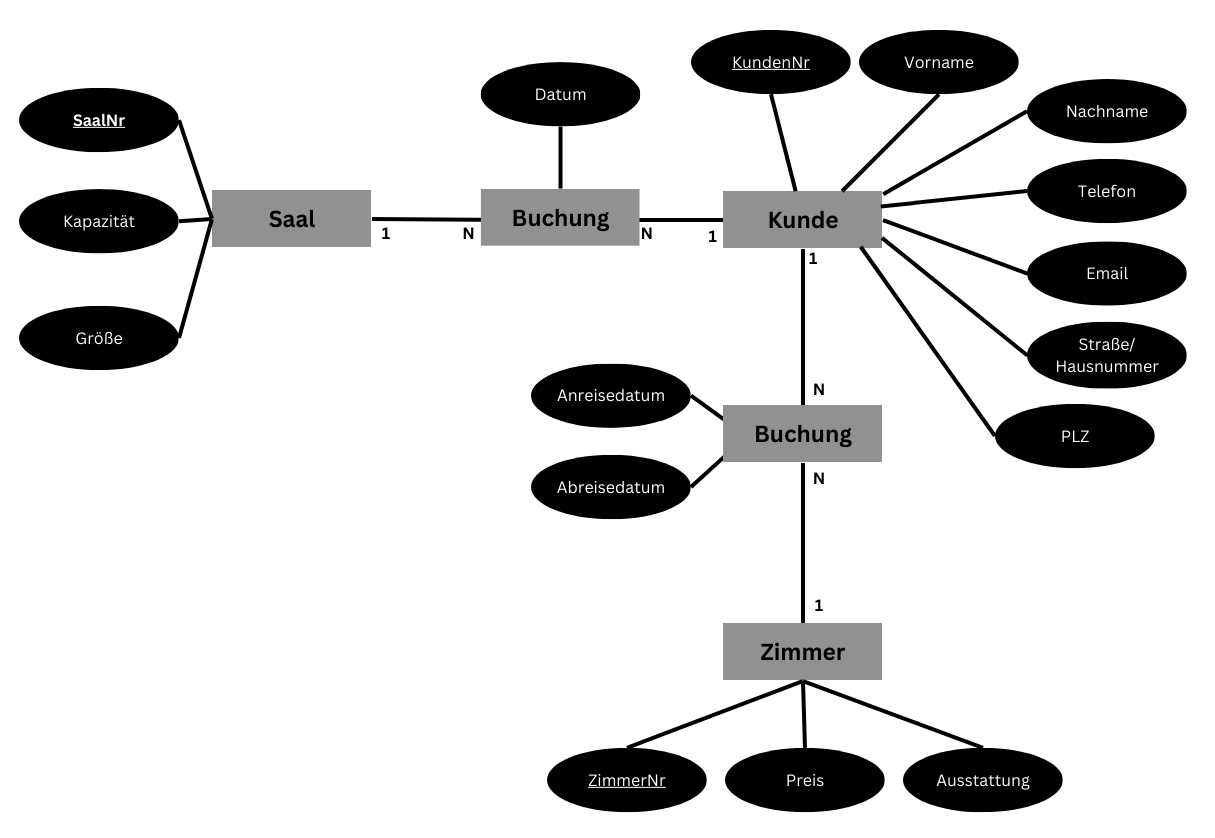
\includegraphics[width=\textwidth]{images/Datenbank.png}
	\caption{Datenbankentwurf}
\end{figure}

Dieser Algorithmus spielt in der finalen Implementierung eine wichtige Rolle, da in vielen Fällen die verfügbaren Zimmer bestimmt werden müssen.
\begin{algorithm}
	\caption{Algorithmus um alle verfügbaren Räume zu erhalten}\label{alg:one}
	\KwData{rooms = alle Räume,
		reservations = alle Buchungen,
		arrival = Anreisedatum,
		departure = Abreisedatum
	}
	\KwResult{available = verfügbare Räume}
	$notAvailable \gets [\thinspace]$; \newline
	\For{room of rooms}{
		\For{reservation of reservations}{
			\If{$(room.id == reservation.room) \thickspace \&\& \thickspace !(departure < reservation.arrival \thickspace || \thickspace arrival > reservation.departure)$}{
				notAvailable.push(room);\newline
				break;
			}
		}
	}

    \Return{$available = rooms.filter(item \thickspace => \thickspace !notAvailable.includes(item))$}
\end{algorithm}